\section{Sauerstoff und Stickstoff Molekülorbitale}
\authors{David Bürg, Ole Simmering}

Im Folgenden betrachten wir das Sauerstoff- und das Stickstoffmolekül im Lichte
der Molekülorbitaltheorie. Bei dieser Betrachtung fällt auf, dass die
Elektronenkonfigurationen der Moleküle sich darin unterscheiden, dass die
antibindenden-$ \pi $-Orbitale beim Sauerstoffmolekül
(siehe Abb. \ref{MO des O2})
einfach und beim Stickstoff (siehe Abb. \ref{MO des N2}) unbesetzt sind.

\begin{dsafigure}
	\centering
	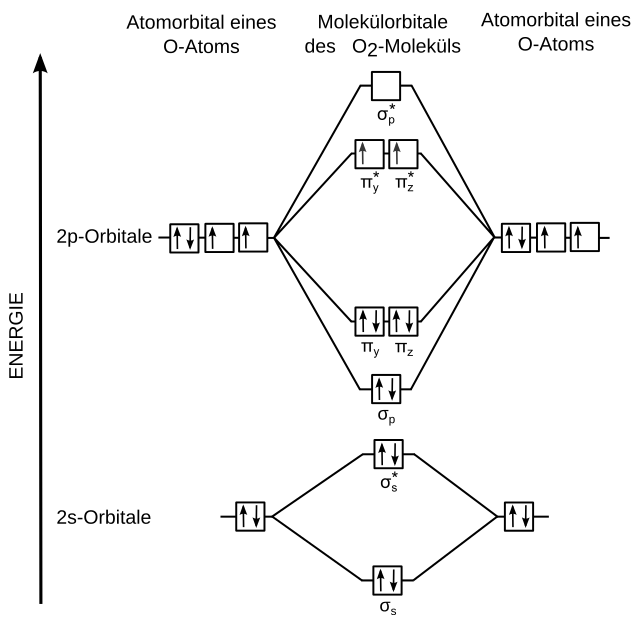
\includegraphics[width=\columnwidth]{MO_O2.png}
	\caption{Molekülorbitaldiagamm eines Sauerstoffmoleküls \cite{MOO2}.}
	\label{MO des O2}
\end{dsafigure}

\begin{dsafigure}
	\centering
	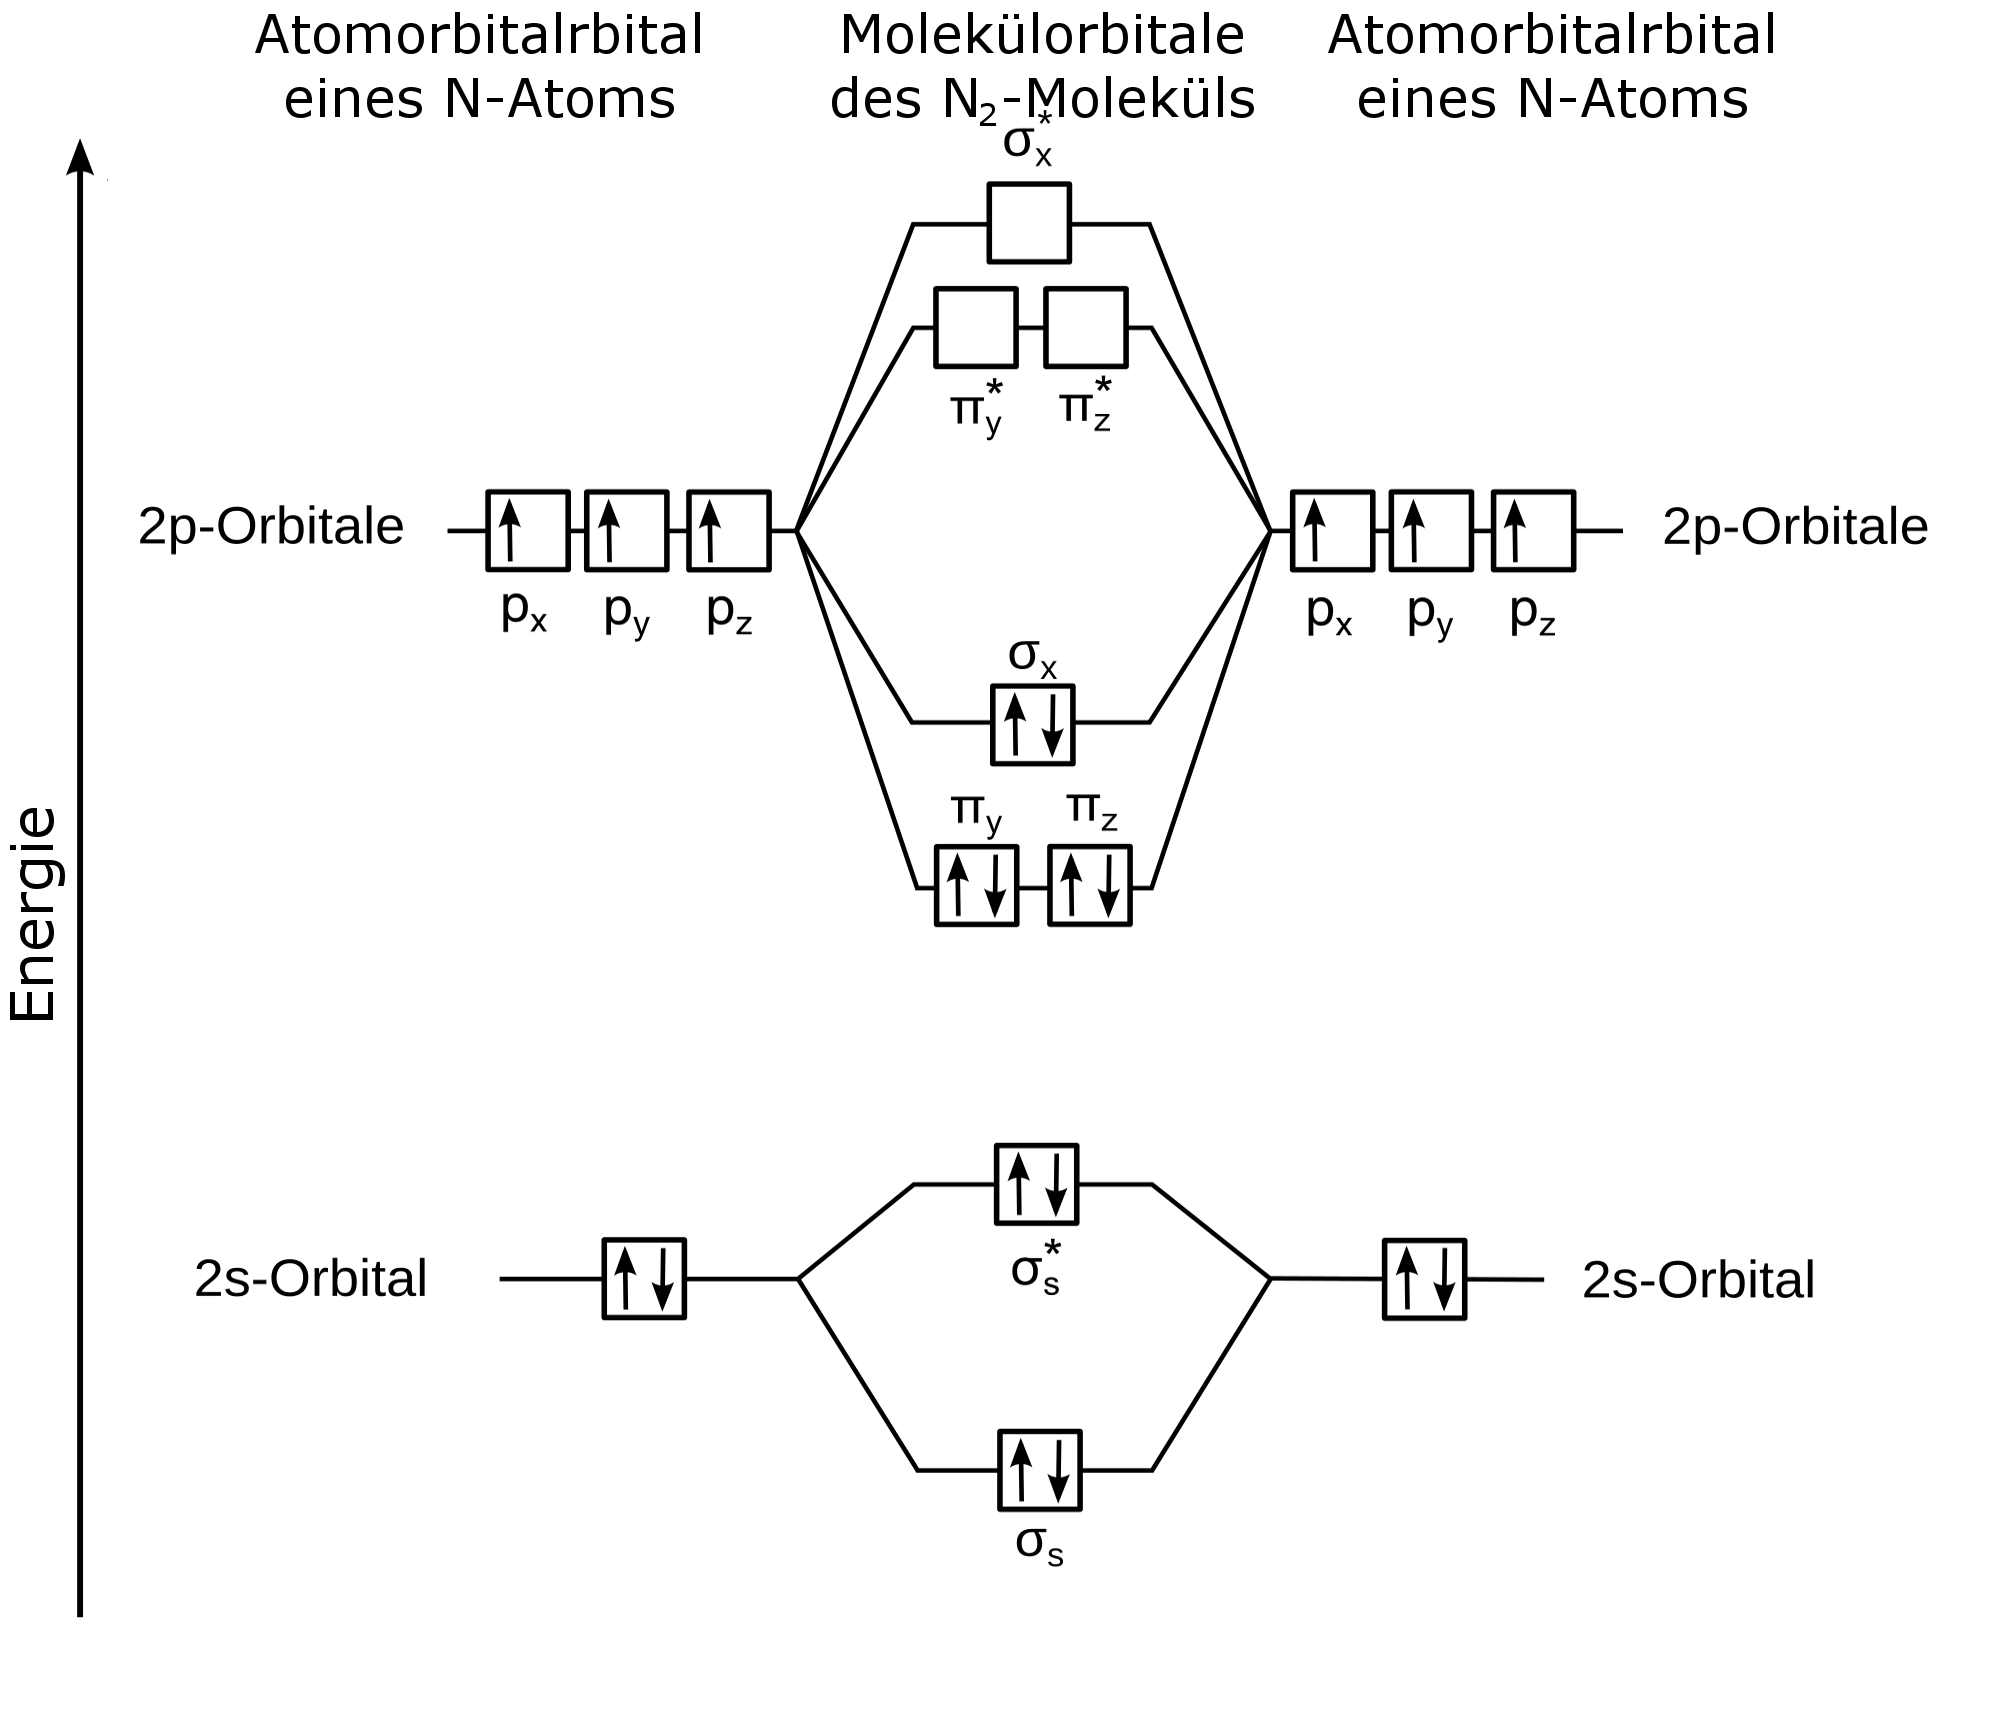
\includegraphics[width=\columnwidth]{MO_stickstoff.png}
	\caption{Molekülorbitaldiagramm eines Stickstoffmoleküls \cite{MON2}.}
	\label{MO des N2}
\end{dsafigure}

Dadurch ist das Sauerstoffmolekül paramagnetisch, hat Radikalcharakter und
befindet sich zudem im Triplettzustand. Bei molekularem Stickstoff ist dies
nicht der Fall. Dieser Umstand ist darauf zurück zu führen, dass das Sauerstoffatom ein Valenzelektron pro Atom mehr aufweist als das Stickstoffatom. Die gerade genannten Eigenschaften können durch eine Berechnung der Elektronenkonfiguration mit dem quantenchemischen Programm ADF \cite{ADF2017authors} feststellt werden. Die Berechnung wurde mit unrestricted DFT (DZ/B3LYP) für Sauerstoff und restricted DFT (DZ/B3LYP) für Stickstoff durchgeführt. Zuletzt wurde zur Optimierung der Struktur eine Kraftfeldoptimierung der Molekülgeometrie vorgenommen. Die Berechnung liefert die Molekülorbitaldiagramme von Sauerstoff [Abb. \ref{MO_O2_levels}] beziehungsweise Stickstoff [Abb. \ref{MO_N2_levels}].


\begin{dsafigure}
	\centering
	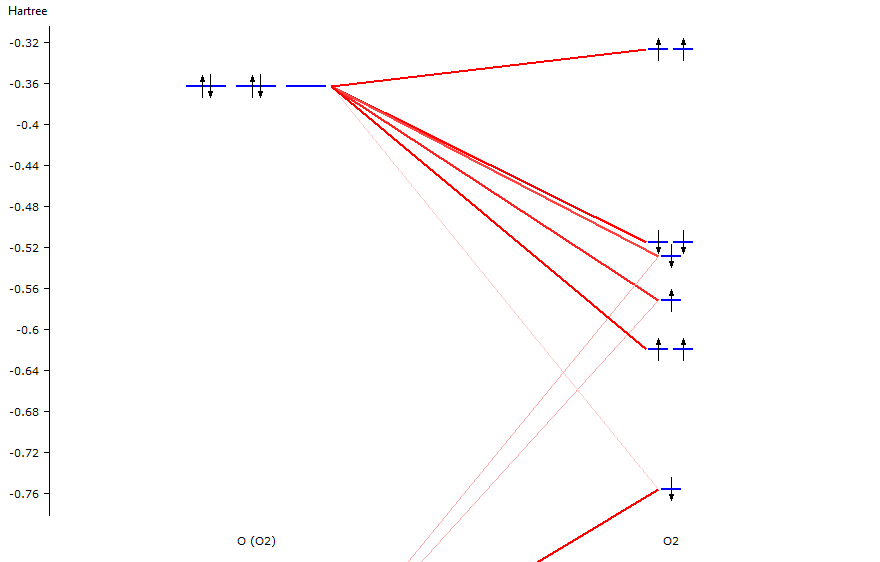
\includegraphics[width=\columnwidth]{MO_O2_levels.png}
	\caption{Mit ADF berechnetes Molekülorbitaldiagramm des Sauerstoffmoleküls.}
	\label{MO_O2_levels}
\end{dsafigure}

\begin{dsafigure}
	\centering
	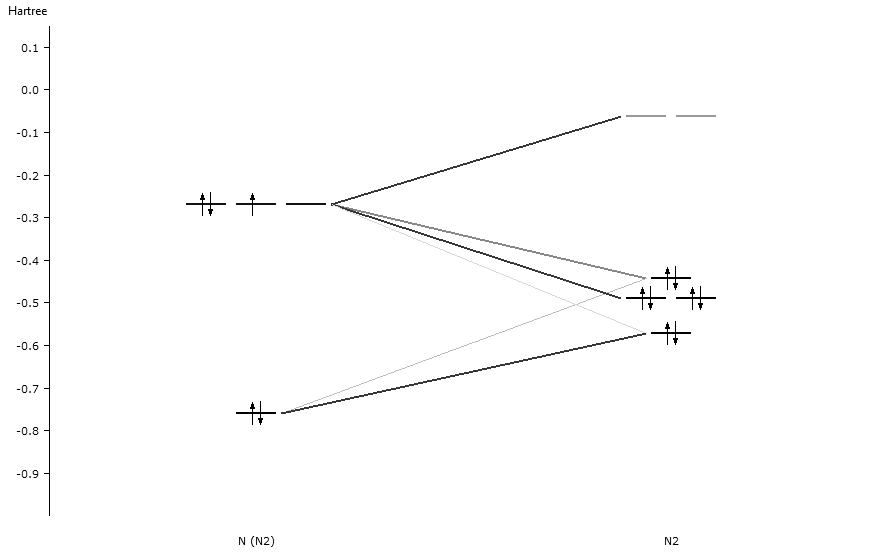
\includegraphics[width=\columnwidth]{MO_N2_levels.png}
	\caption{Mit ADF berechnetes Molekülorbitaldiagramm des Stickstoffmoleküls.}
	\label{MO_N2_levels}
\end{dsafigure}
